% Chapter 1: Thesis Introduction
% This chapter provides an introduction to the thesis, including key definitions,
% research questions, and a summary of included papers.

\section{Introduction}
\subsection{Overview}
% TODO: Add overview content
% This section should provide a high-level overview of the thesis topic,
% its significance, and the overall contribution to the field.

% TODO: Add content for the overview section

\section{Key Definitions}
% TODO: Add key definitions content
% This section should define important terms, concepts, and methodologies
% that are central to the thesis work.

% TODO: Add content for key definitions

\section{List of Abbreviations}
% TODO: Add list of abbreviations content
% This section should provide a comprehensive list of abbreviations
% used throughout the thesis.

% TODO: Add content for list of abbreviations

\section{Research Question}
\subsection{Aims \& Objectives}
The objective of this research is to enhance formal verification in industrial automation by incorporating modular nondeterministic transitions (NDTs) to improve realism and complexity management. It aims to develop modular applications with automatic verification procedures and automate plant model generation within IEC 61499 for formal verification. Additionally, the research focuses on creating portable test codes for cross-platform validation to ensure consistency in different runtime environments. To further optimize industrial automation, the study integrates AI agents to enable reasoning, planning, and real-time adaptability of IEC 61499-based control systems.

\subsection{Hypothesis}
This research hypothesizes that integrating formal verification techniques with modular automation frameworks enhances system reliability and scalability, while non-deterministic transitions enable realistic simulation and validation of complex processes. Process mining can extract control logic from event logs, enabling automated model generation for verification and analysis. Automated test generation improves system portability and validation, ensuring reliable cross-platform performance. AI-driven agents, leveraging knowledge graphs and LLMs, enhance industrial automation by enabling sustainable planning, dynamic execution, and requirement-based validation of IEC 61499 control systems through OPC UA integration.

\subsection{Problem Statement}
Integrating formal verification into the design of IEC 61499-based automation systems remains a challenge in ensuring reliability and correctness. Leveraging process mining to generate formal models from event logs can improve system analysis, but effective methods for this transformation are needed. Detecting portability issues before deployment is critical to prevent failures due to execution environment differences. AI-driven reasoning, planning and decision-making can enhance system adaptability, but efficient implementation methods need further exploration.

\subsection{Research Questions}
\subsubsection{Main Research Question}
How can best practices in formal verification, process mining, model-based testing, and AI-driven automation be combined to enhance the safety, conformance, portability and adaptability of industrial control systems?

\subsubsection{Sub-questions}
\begin{enumerate}
    \item How can formal verification techniques be applied to modular industrial automation systems to ensure their safety and correctness?
    
    \item How can the plant model creation be automated by process mining? How could such models be integrated into the formal verification toolchain to verify and optimize industrial control systems based on IEC 61499?
    
    \item How can model-based testing improve the portability and reliability of IEC 61499 control applications across multiple platforms?
    
    \item How can a knowledge-driven AI agent interpret natural-language operator instructions to generate sustainable execution plans for IEC 61499-based industrial control systems? How can AI agents automate requirement-based testing and validate system behavior to ensure conformance in industrial control systems?
\end{enumerate}

\section{Included Papers' Summary}
The following section lists all publications included in Part II of the thesis. A short summary of each paper is presented and my contribution is highlighted. Figure~\ref{fig:ch1:research_mapping} shows the mapping between papers appended and what research question they address and Figure~\ref{fig:ch1:paper_relationship} shows how the appended papers are linked to achieving the thesis objective.

\begin{figure}[htbp]
    \centering
    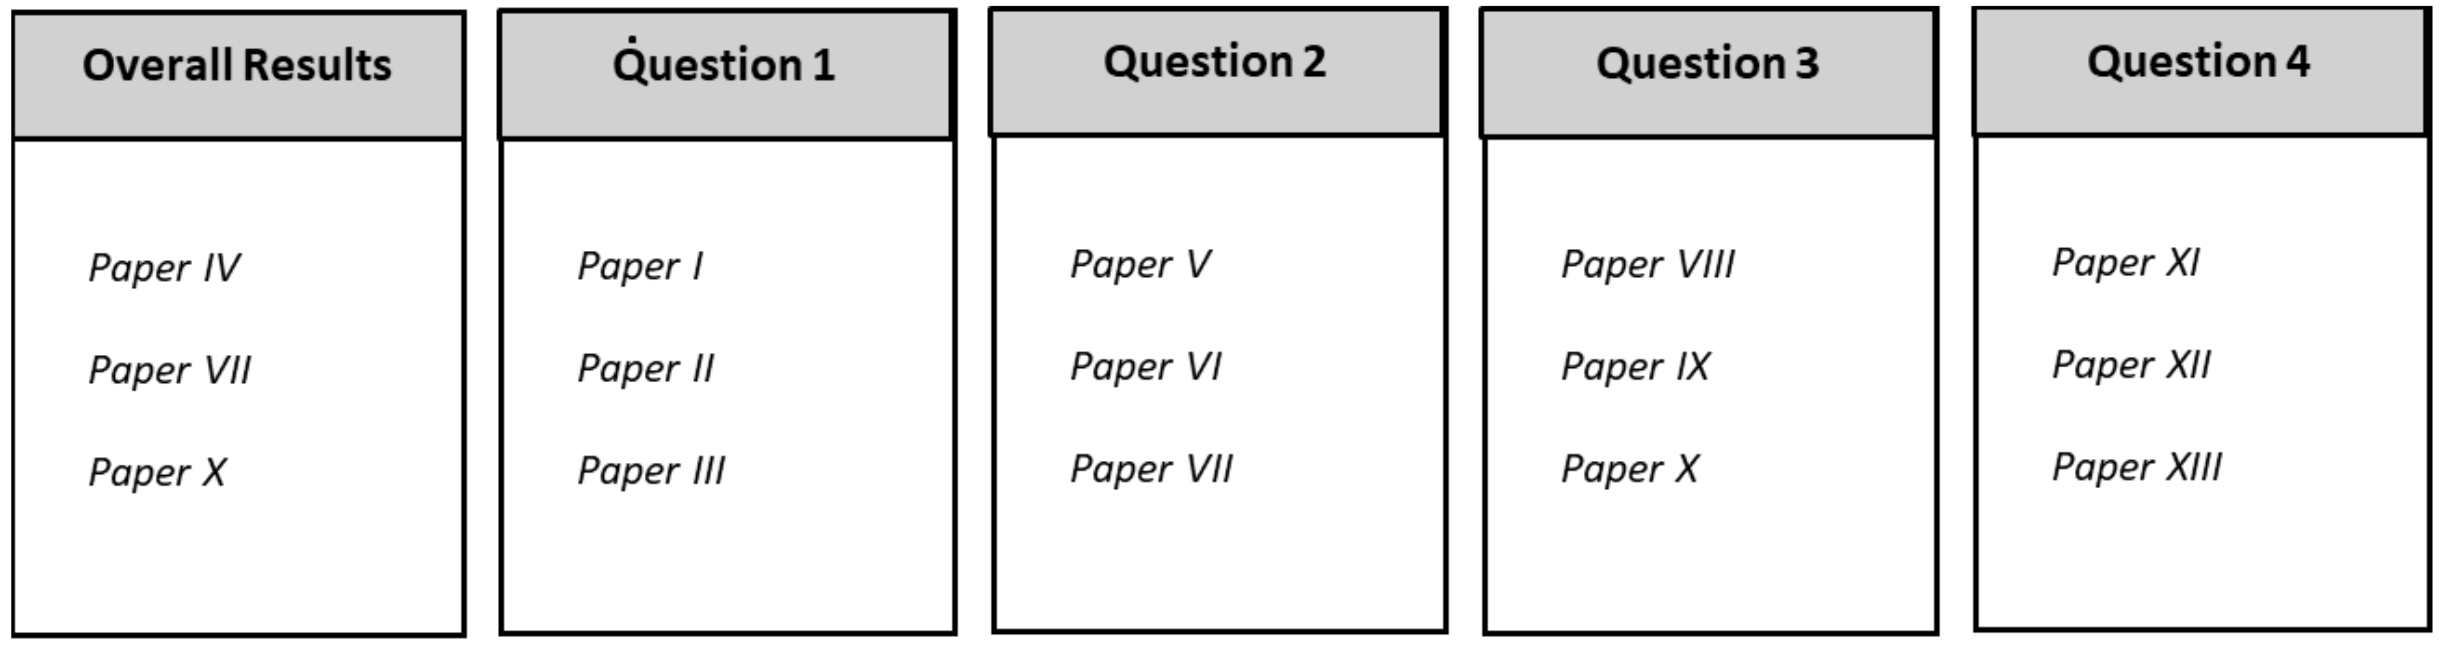
\includegraphics[width=0.9\textwidth]{chapters/images/chapter1/relationship_papers_researchquestions.png}
    \caption{Mapping between research questions and appended papers.}
    \label{fig:ch1:research_mapping}
\end{figure}

\begin{figure}[htbp]
    \centering
    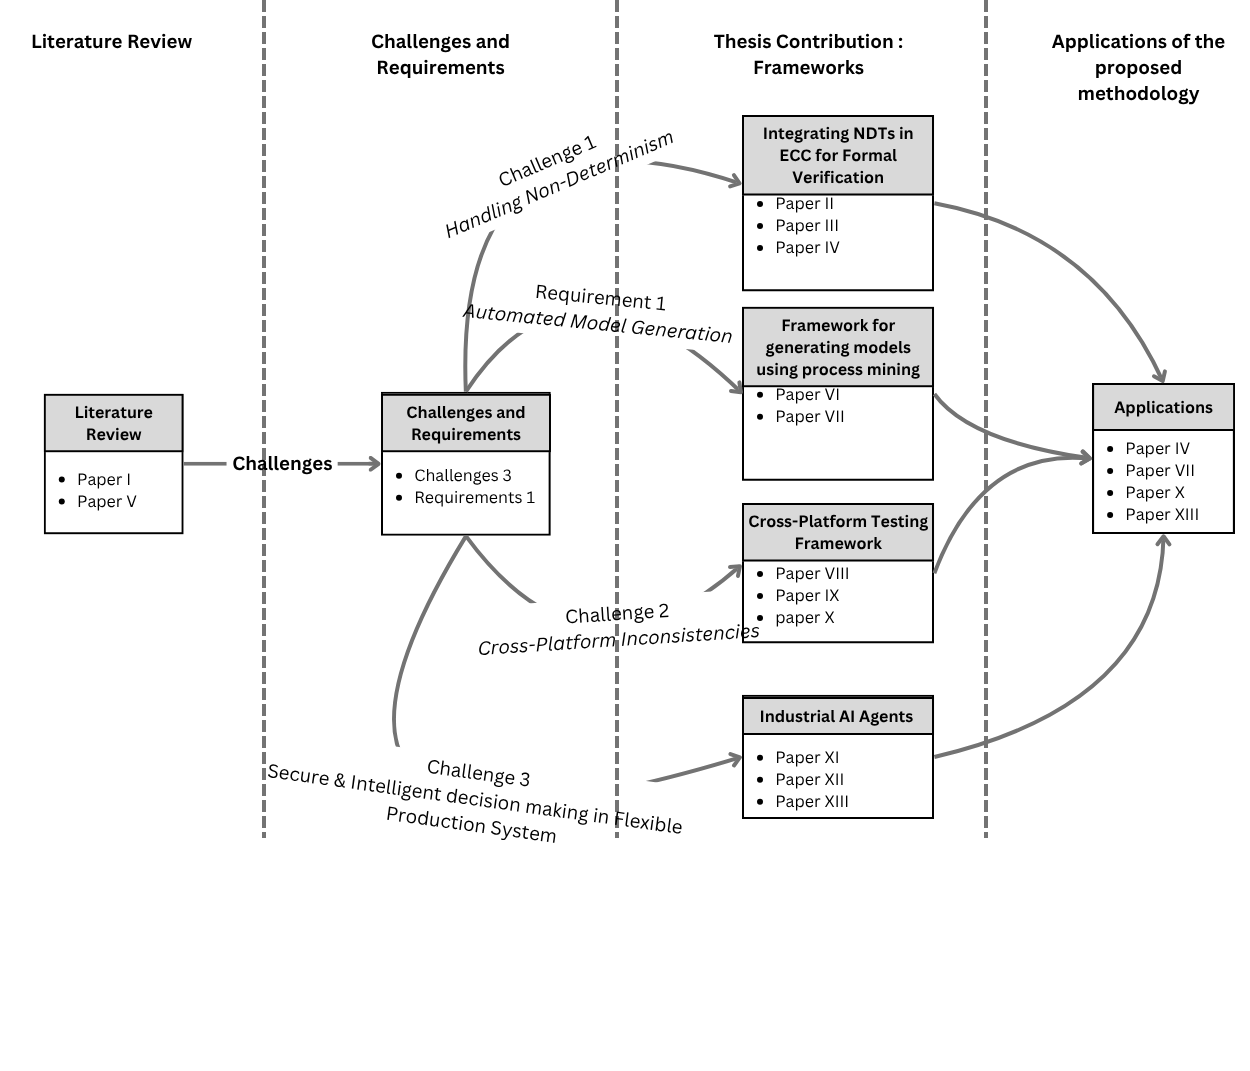
\includegraphics[width=0.9\textwidth]{chapters/images/chapter1/Literature Review.png}
    \caption{Relation between appended papers and the thesis topics.}
    \label{fig:ch1:paper_relationship}
\end{figure}

% TODO: Add detailed summaries of each included paper
% This section should provide a brief summary of each included paper,
% highlighting their contributions and how they relate to the overall thesis.

% TODO: Add content for individual paper summaries
